%% Copyright 2019 Bernd Haberstumpf
%% License: CC BY-NC
% !TeX spellcheck = de_DE
\newsection{Kampf und Verletzungen}

Im Alltag eines Helden l"asst sich eine Auseinandersetzung nicht immer friedlich l"osen, und es kommt zum Kampf. In diesem Kapitel werden K"ampfe zwischen Personen und die Auswirkungen von Verletzungen beschrieben.

Eine Aktion in einem Kampf umfasst eine ganze \emph{Kampfszene}. Eine solche Kampfszene kann z.B. ein Nahkampfgefecht, ein Schusswechsel oder auch ein Ausweichman"over sein. Der Spieler beschreibt, wie er k"ampfen m"ochte und welches Ziel er in der Kampfszene erreichen m"ochte: M"ochte er einen oder mehrere Gegner mit Tritten zu Fall bringen, in Deckung hechten oder einen fl"uchtenden Gegner niederschie\3en?

Daraufhin wird gew"urfelt. K"ampfe sind normalerweise \textbf{vergleichende W"urfe} mit der Schwierigkeit \textbf{Einfacher Wurf}. Entschlie\3t sich ein Charakter, seinen Gegner \textbf{anzugreifen}, w"urfelt er mit seiner F"ahigkeit \textbf{Fight}. Beschr"ankt sich der Charakter auf \textbf{Verteidigung}, wird je nach Situation entweder mit \textbf{Fight} oder \textbf{Agility} gew"urfelt. Auf \textbf{Agility} wird gew"urfelt, wenn der Charakter einem Angriff ausweichen will.

\begin{ruleexample}
    Hektor und der Minenarbeiter Fury, ein kr"aftiger Alpha-Mutant, sind aneinander geraten. Fury schl"agt zu. Hektor sieht sich unterlegen und versucht zu fliehen.

    Fury w"urfelt auf \stat{Fight}. Hektors w"ahlt \stat{Agility}. Beide haben zwei W"urfel zur Verf"ugung. Im Rahmen eines vergleichenden Wurfs w"urfelt Fury mit einem W"urfel und erzielt eine \ssdice{4}, Teilerfolg. Furys Schl"age sind kr"aftig und gut gezielt, aber Hektor schafft es immer wieder, gekonnt abzutauchen, und steckt nur leichte Treffer ein.

    Hektor versucht, sich aus dem Kampf zu l"osen und die Flucht anzutreten. Er w"urfelt mit \stat{Agility}, reduziert durch Furys Angriffswert \stat{Fight}. Er w"urfelt ebenfalls mit einem W"urfel und erzielt eine \ssdice{5}, Teilerfolg. Hektor bringt sich auf Abstand und entscheidet sich, Fury zu beruhigen.
\end{ruleexample}

\newsubsection{Kampf mit mehreren Personen}
Oft sind an K"ampfen mehrere Personen beteiligt. Wie bei anderen Aktionen k"onnen Angreifer oder Verteidiger ihre Kr"afte b"undeln, um ihre Erfolgschancen zu erh"ohen. Das B"undeln wird \cref{sec:bundleforce}. Sowohl die Angreifer als auch die Verteidiger k"onnen ihre W"urfel b"undeln.

\newsubsection{Nahkampf}
Im Nahkampf treten Personen waffenlos oder mit Hieb- oder Stichwaffen gegeneinander an.

Im Folgenden sind einige spezielle Nahkampfsituationen beschrieben:

\begin{description}
    \item[Fixieren] Ein Angriff, um einen Gegner festzuhalten und bewegungsunf"ahig zu machen. Der Gegner ist dann kampfunf"ahig, kann sich 
        jedoch m"oglicherweise in einer sp"ateren Kampfszene befreien. Um einen Gegner zu fixieren, wird ein \textbf{voller Erfolg} ben"otigt. Ein Teilerfolg k"onnte bedeuten, dass der Gegner zwar nicht fl"uchten kann, aber noch nicht vollst"andig kampfunf"ahig ist.
    \item[Entwaffnen] Dem Gegner eine Waffe zu entrei\3en oder sie ihm zu entwinden, erfordert einen \textbf{vollen Erfolg}. Ein Teilerfolg 
        kann den Schaden des Angriffs verringern.
    \item[Schl"agerei] An einer Schl"agerei k"onnen viele Personen beteiligt sein. Aufgrund der Enge, k"onnen jedoch immer maximal drei 
        Personen ihre Angriffe b"undeln.
\end{description}

\newsubsection{Fernkampf}
Fernkampf bezieht sich auf Angriffe mit Wurfwaffen, Schusswaffen, Granaten und Plasmaschleudern. Der Angreifer w"urfelt mit der F"ahigkeit \stat{Fight}, um anzugreifen.

Folgende Besonderheiten m"ussen ber"ucksichtigt werden:

\begin{description}
    \item[Ausweichen] Um einem Fernkampfangriff auszuweichen, muss der Verteidiger in der Regel bereits in Bewegung sein, Haken schlagen 
        oder in Deckung hechten. Um auf einen Fernkampfangriff zu reagieren, wird mit der F"ahigkeit \textbf{Agility} gew"urfelt.
    \item[Duell] Ein Angreifer, der eine Fernkampfwaffe nutzt, kann normalerweise anderen Angriffen kaum ausweichen. Um dennoch auf 
        einen Gegenangriff zu reagieren, ist ein \textbf{Risikowurf} erforderlich.
    \item[Point-Blank] Ein Angreifer, der einen Gegner ohne Deckung aus kurzer Distanz bedroht, hat leichtes Spiel. Er w"urfelt seinen 
        Angriff mit einem \textbf{Alltagswurf}. Der Angegriffene kann entweder einen Nahkampf-Gegenangriff versuchen oder sich mit einer schnellen Bewegung aus der Schusslinie bringen, wenn ihm der Sch"utze Auge-in-Auge gegen"ubersteht. In diesem Fall w"urfelt er einen \textbf{Risikowurf} als Gegenreaktion.
    \item[Deckung] Ein Verteidiger, der in teilweiser Deckung steht, ist schwerer zu treffen. Die Verteidigung erh"alt einen \textbf{Bonus}  
        von einem W"urfel, sofern die R"ustung diesen Bonus nicht bereits bietet.
\end{description}

\newsubsection{Schaden}\anchor{sec:schaden}
Bei K"ampfen und auch in anderen Situationen kann ein Charakter verletzt werden. Verletzungen werden nicht wie in anderen Rollenspielen durch Lebenspunkte festgehalten. Stattdessen bestimmt der Spielleiter basierend auf dem Angriff, der Verteidigung, der Panzerung sowie den Umst"anden, die zur Verletzung f"uhren, welche Art von Verletzung der Charakter erleidet. Die Auswirkung einer Verletzung legt der Spielleiter fest.

\begin{column}[l]{0.58}
    Wird der Charakter im Kampf oder bei einer sonstigen T"atigkeit verletzt, wird unter \stat{DAMAGE} die zugezogene Verletzung notiert. Es wird zwischen \textbf{leichtem} und \textbf{schwerem Schaden} unterschieden. Bei schweren Verletzungen ist ein Konstitutionswurf notwendig, damit der Charakter handlungsf"ahig bleibt. Werden schwere Sch"aden nicht behandelt oder setzt sich der Charakter weiterhin k"orperlicher Belastung aus, kann er ebenfalls handlungsunf"ahig werden. In diesem Fall k"onnen weitere Konstitutionsw"urfe erforderlich werden. Ein Konstitutionswurf ist in der Regel ein \textbf{einfacher Wurf} auf \stat{CONST}.
\end{column}
\begin{column}[r]{0.42}
    \centering
    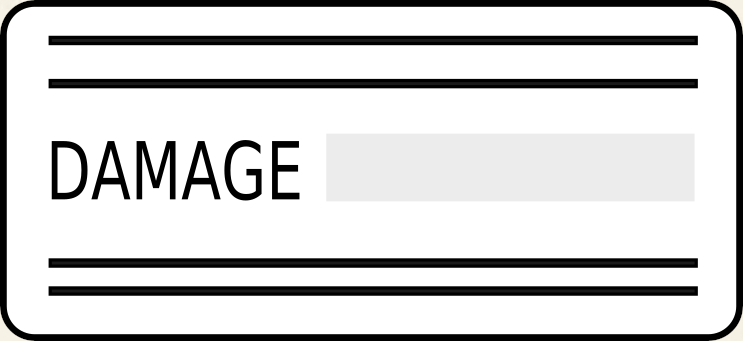
\includegraphics[width=0.80\textwidth]{images/character_damage.jpg}

    
\includegraphics[width=0.80\textwidth]{images/character_const.jpg}
\end{column}
\smallskip

Schwere Verletzungen in Verbindung mit einem erfolglosen Konstitutionswurf k"onnen zum Tod f"uhren. Die Verletzung muss sofort behandelt werden, andernfalls f"uhrt sie unweigerlich zum Exitus. Ein sterbender Charakter kann jedoch wiederbelebt werden. Die Medizin im 23. Jahrhundert ist, wie \cref{sec:helden} beschrieben, weit fortgeschritten. K"orpermodifikationen k"onnen dabei helfen, den Charakter am Leben zu halten. Ein Erste-Hilfe-Kit enth"alt Ausr"ustung zur Wiederbelebung und Stabilisierung.

\newsubsection{Kleine, Leichte, schwere und Bet"aubungswaffen}\anchor{sec:heavyweapons}

Im Rahmen des Regelwerks wird zwischen kleinen, leichten und schweren Waffen unterschieden.

\begin{description}
    \item [Kleine Waffen] Unter kleinen Waffen werden alle Nahkampfwaffen und Handfeuerwaffen verstanden. Alle Panzerungen im n"achsten 
        Kapitel \cref{sec:panzerung} bieten effektiven Schutz gegen kleine Waffen.
    \item[Leichte Waffen] Unter leichte Waffen fallen vollautomatische Gewehre wie Railguns und Handgranaten. Gegen leichte Waffen bieten 
        Panzerungen, au\3er einem Servopanzer, nur begrenzten Schutz.
    \item[Schwere Waffen] Unter schwere Waffen fallen Plasmaschleudern, Granatwerfer, Raketenwerfer und alle Fahrzeug-gest"utzten 
        Waffensysteme. Auch ein Teiltreffer ist in den meisten F"allen fatal. Nur ein Servopanzer bietet Schutz gegen einen indirekten Treffer (Teilerfolg).
    \item[Bet"aubungswaffen] Unter Bet"aubungswaffen versteht man Waffen, die einen Gegner au\3er Gefecht setzen, ohne ihn schwer zu 
        verwunden.
        
        Eine effektive Munition dieser Kategorie sind Schockprojektile. Hierbei handelt es sich um nicht penetrierende Projektile, die beim Aufprall auf das Ziel kurzzeitig einen starken Stromsto\3 abgeben, der zu Muskelkr"ampfen, Bewusstlosigkeit und zum Ausfall von elektronischen Ger"aten wie Cyberware f"uhren kann. Gegen Schockprojektile bietet nur ein Servopanzer effektiven Schutz. Andere Panzerungen bieten nur begrenzten Schutz.
\end{description}

\underline{Anmerkung:} Die hier verwendeten Begriffe entsprechen nicht den offiziellen Bezeichnungen der UN.

\newsubsection{Panzerung}\anchor{sec:panzerung}
Um sich gegen Angriffe zu sch"utzen, kommt Panzerung ins Spiel. Eine Panzerung sch"utzt recht zuverl"assig vor kleinen Waffen. Kritisch sind ungesch"utzte K"orperteile.

Folgende Panzerungen kommen im C23-Universum zum Einsatz:

\begin{description}
    \item[Schusssichere Weste und Helm] Eine schusssichere Weste und ein Helm bieten bereits einen effektiven Schutz gegen kleine Waffen. Sie sch"utzen den Torso und Teile des Kopfes effektiv vor Stichwaffen und Projektilen und bieten auch Schutz gegen stumpfen Waffen. Ein Treffer auf Weste und Helm hinterl"asst Prellungen, verursacht jedoch keine gr"o\3eren Verletzungen. Ein Treffer auf ungesch"utzte K"orperteile erfordert einen \textbf{vollen Erfolg}.
    \item[Kampfanzug] Noch besseren Schutz bietet ein Kampfanzug. Ein Kampfanzug sch"utzt alle Teile des K"orpers, aber er bietet auch     
        keinen vollst"andigen Schutz vor kleinen und leichten Waffen oder Schl"agen. Bewegliche Teile wie Gliedma\3en sind nach wie vor weniger gut gesch"utzt. Nur ein \textbf{herausragender Erfolg} trifft ein schlecht gesch"utztes K"orperteil.
    \item[Servopanzer] Ein Servopanzer ist ein hydraulisch unterst"utztes Ganzk"orper-Exoskelett mit eingebautem Raumanzug und 
        Waffensystemen. Treffer mit einer Nahkampfwaffe oder einer kleinen Waffe sind bei einem Servopanzer wirkungslos. Selbst die schw"acher gesch"utzten K"orperteile bieten eine Schutzwirkung, die mit einer schusssicheren Weste vergleichbar ist.
\end{description}

